\section{Synchronisation et parallélisme dynamique}
\begin{frame}
    \frametitle{Flux de synchronisation}
\begin{block}{Opérations asynchrones}
    \begin{itemize}
        \item<+-> Par défaut, les exécutions de noyaux sur le GPU sont indépendantes du déroulement
        du programme sur CPU, sauf pour les transferts mémoire ou les lancements de grilles de processus.
        \item<+-> Dans de nombreux cas, il pourrait être bénéfique de s'affranchir de cette limitation.
        \item<+-> Les flux d'exécution ont été introduits pour permettre à des noyaux différents ou à des opérations
        de transfert entre hôte et GPU de se dérouler concurremment. 
    \end{itemize}
\end{block}
\end{frame}
\begin{frame}[fragile]
    \frametitle{Flux de synchronisation}
\begin{block}{Transferts mémoire asynchrones}
    \begin{itemize}
        \item<+-> Un flux d'exécution est créé par un appel à la fonction \texttt{cudaStreamCreate(cudaStream\_t *stream)}
        \item<+-> Il est supprimé en appelant \texttt{cudaStreamDestroy(cudaStream\_t stream)}
        \item<+-> Un transfert mémoire associé à un flux est réalisé à l'aide de la fonction \texttt{cudaMemcpyAsync()}.
        \item<+-> Il est indépendant de l'ordre d'appel sur l'hôte, mais est synchronisé sur le flux.
        \item<+-> Les transferts de mémoire asynchrones ne peuvent s'effectuer qu'entre des blocs spécifiquement alloués sur l'hôte par 
        \texttt{cudaMallocHost(void **ptr, size\_t size)}
    \end{itemize}
\end{block}
\end{frame}
\begin{frame}[fragile]
    \frametitle{Flux de synchronisation}
\begin{block}{Grilles de calcul asynchrones}
    \begin{itemize}
        \item<+-> Le dernier paramètre lors du lancement d'une grille de calcul est un flux d'exécution.
        \item<+-> Pour exécuter un noyau \texttt{kernel} dans le flux \texttt(stream) on écrira:
        \texttt{kernel<<<grid,block,dynSharedSize,stream>>>(args)}.
        \item<+-> Les opérations d'un flux se synchronisent sur le flux par défaut, qui est utilisé lorsque le paramètre de flux est absent. Ce comportement peut toutefois être changé.
    \end{itemize}
\end{block}
\end{frame}
\begin{frame}
    \frametitle{Flux de synchronisation}
\begin{block}{Un exemple: le produit scalaire}
    \begin{itemize}
        \item<+-> Le produit scalaire entre deux vecteurs peut être efficacement implémenté sur le GPU.
        \item<+-> Dans cet exemple, on choisit de réaliser un calcul par blocs, mais d'effectuer la réduction sur 
        le CPU.
        \item<+-> On calcule des produits scalaires de façon asynchrone, dans des processus (CPU) différents.
    \end{itemize}
\end{block}
\end{frame}
\begin{frame}
    \frametitle{Noyau pour le produit scalaire}
\begin{block}{Code}
   \begin{tabular}{cc}
        \begin{minipage}{0.45\textwidth}
 \begin{figure}[htbp]
    \centering
   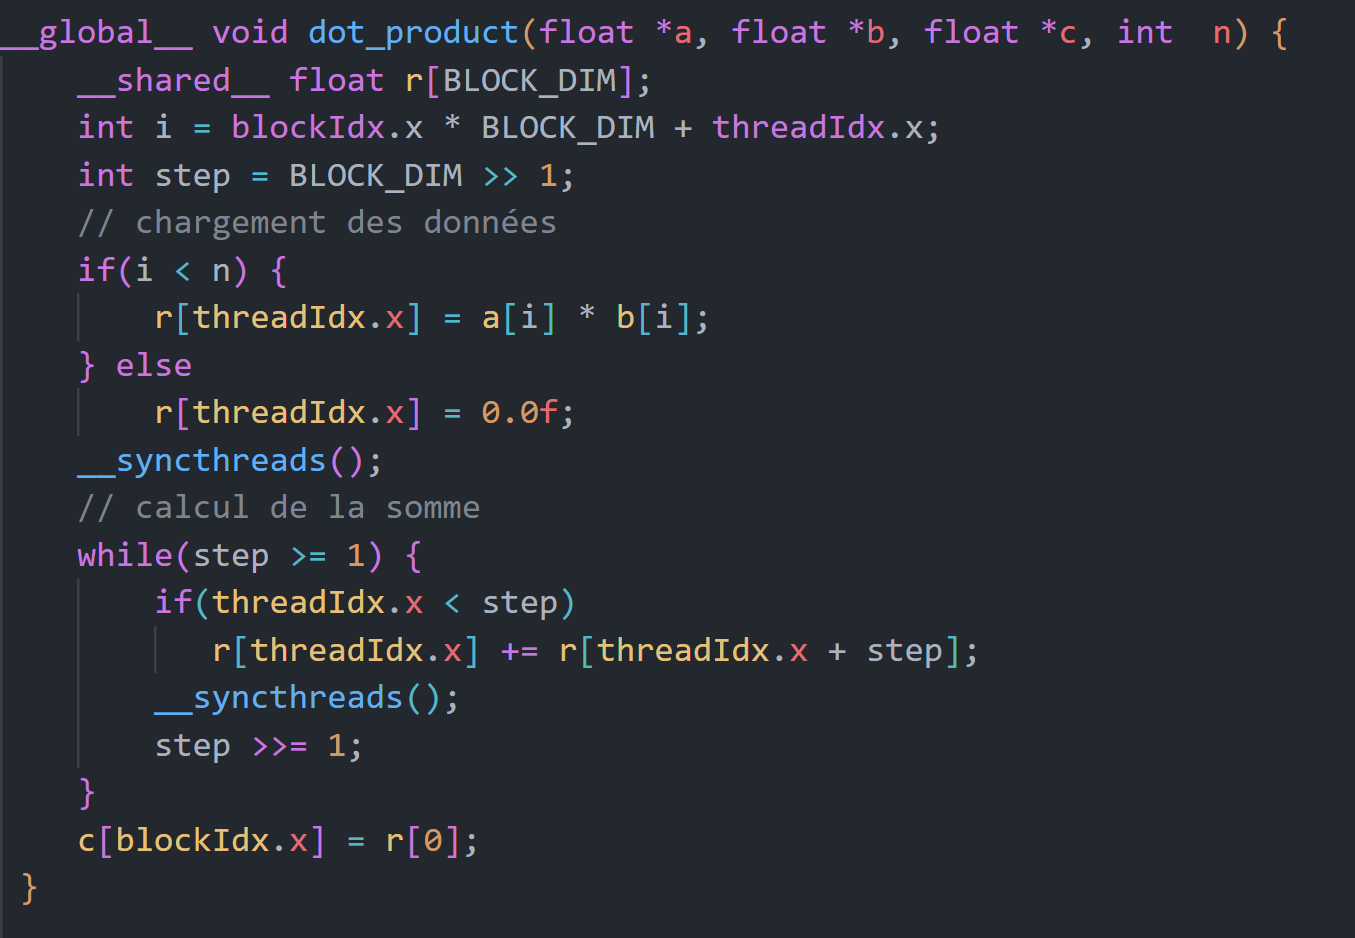
\includegraphics[width=\textwidth]{device_dot.png}
    \caption{Produits partiels sur GPU}
    \label{fig:device_dot}
\end{figure}
        \end{minipage} & 
        \begin{minipage}{0.45\textwidth}
            \begin{itemize}
                \item<+-> La première partie du calcul est classique.
                \item<+-> La réduction s'effectue par sommation d'éléments deux à deux.
           \end{itemize}
        \end{minipage}
\end{tabular}
\end{block}
\end{frame}
\begin{frame}
    \frametitle{Lancement asynchrone}
\begin{block}{Code}
   \begin{tabular}{cc}
        \begin{minipage}{0.45\textwidth}
 \begin{figure}[htbp]
    \centering
   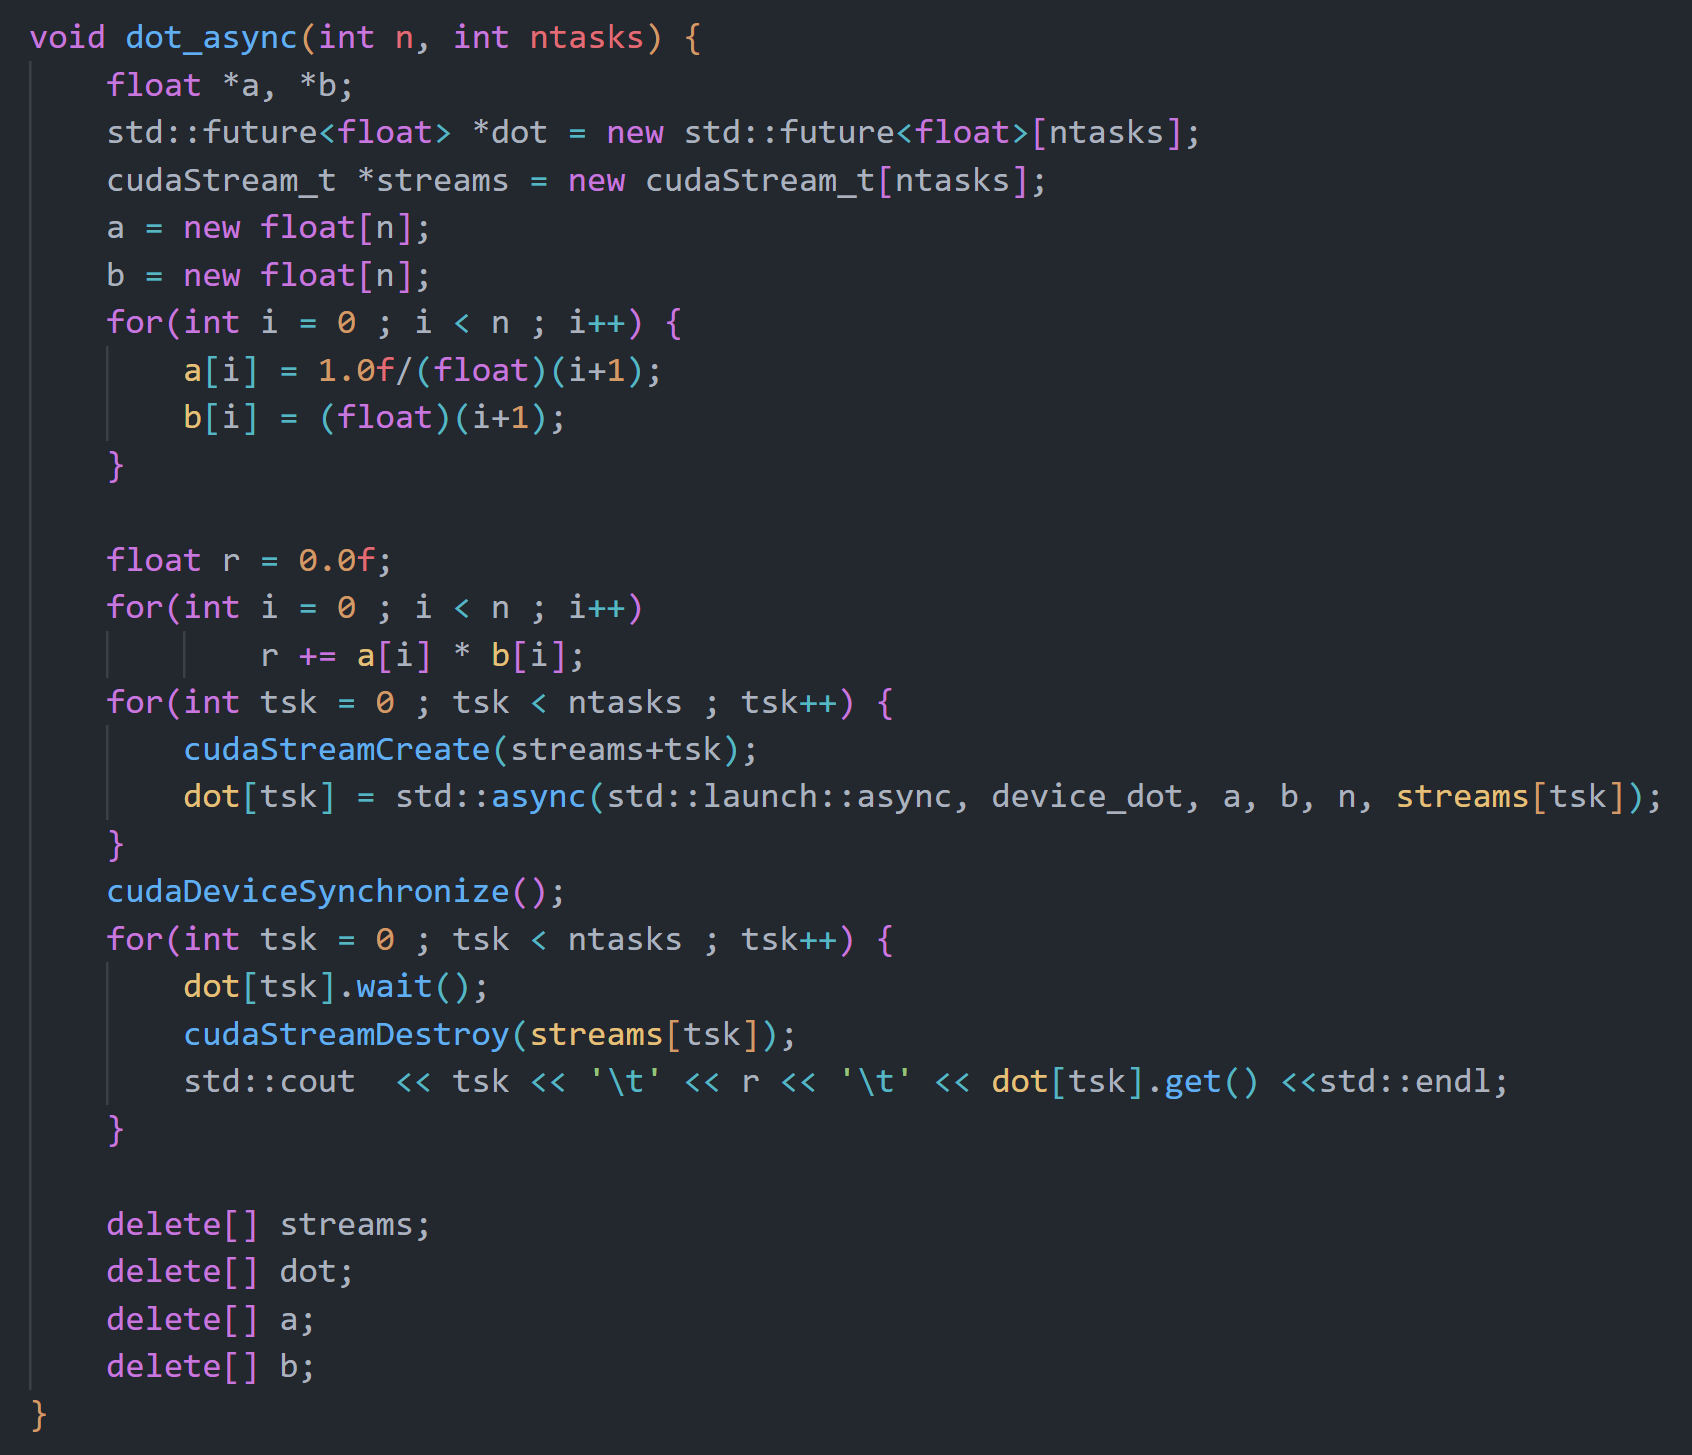
\includegraphics[width=\textwidth]{host_dot.png}
    \caption{API asynchrone.}
    \label{fig:host_dot}
\end{figure}
        \end{minipage} & 
        \begin{minipage}{0.45\textwidth}
            \begin{itemize}
                \item<+-> Les transferts en mémoire et les appels de grille sont attachés à un flux.
           \end{itemize}
        \end{minipage}
\end{tabular}
\end{block}
\end{frame}
\begin{frame}
    \frametitle{Processus de calcul}
\begin{block}{Code}
   \begin{tabular}{cc}
        \begin{minipage}{0.45\textwidth}
 \begin{figure}[htbp]
    \centering
   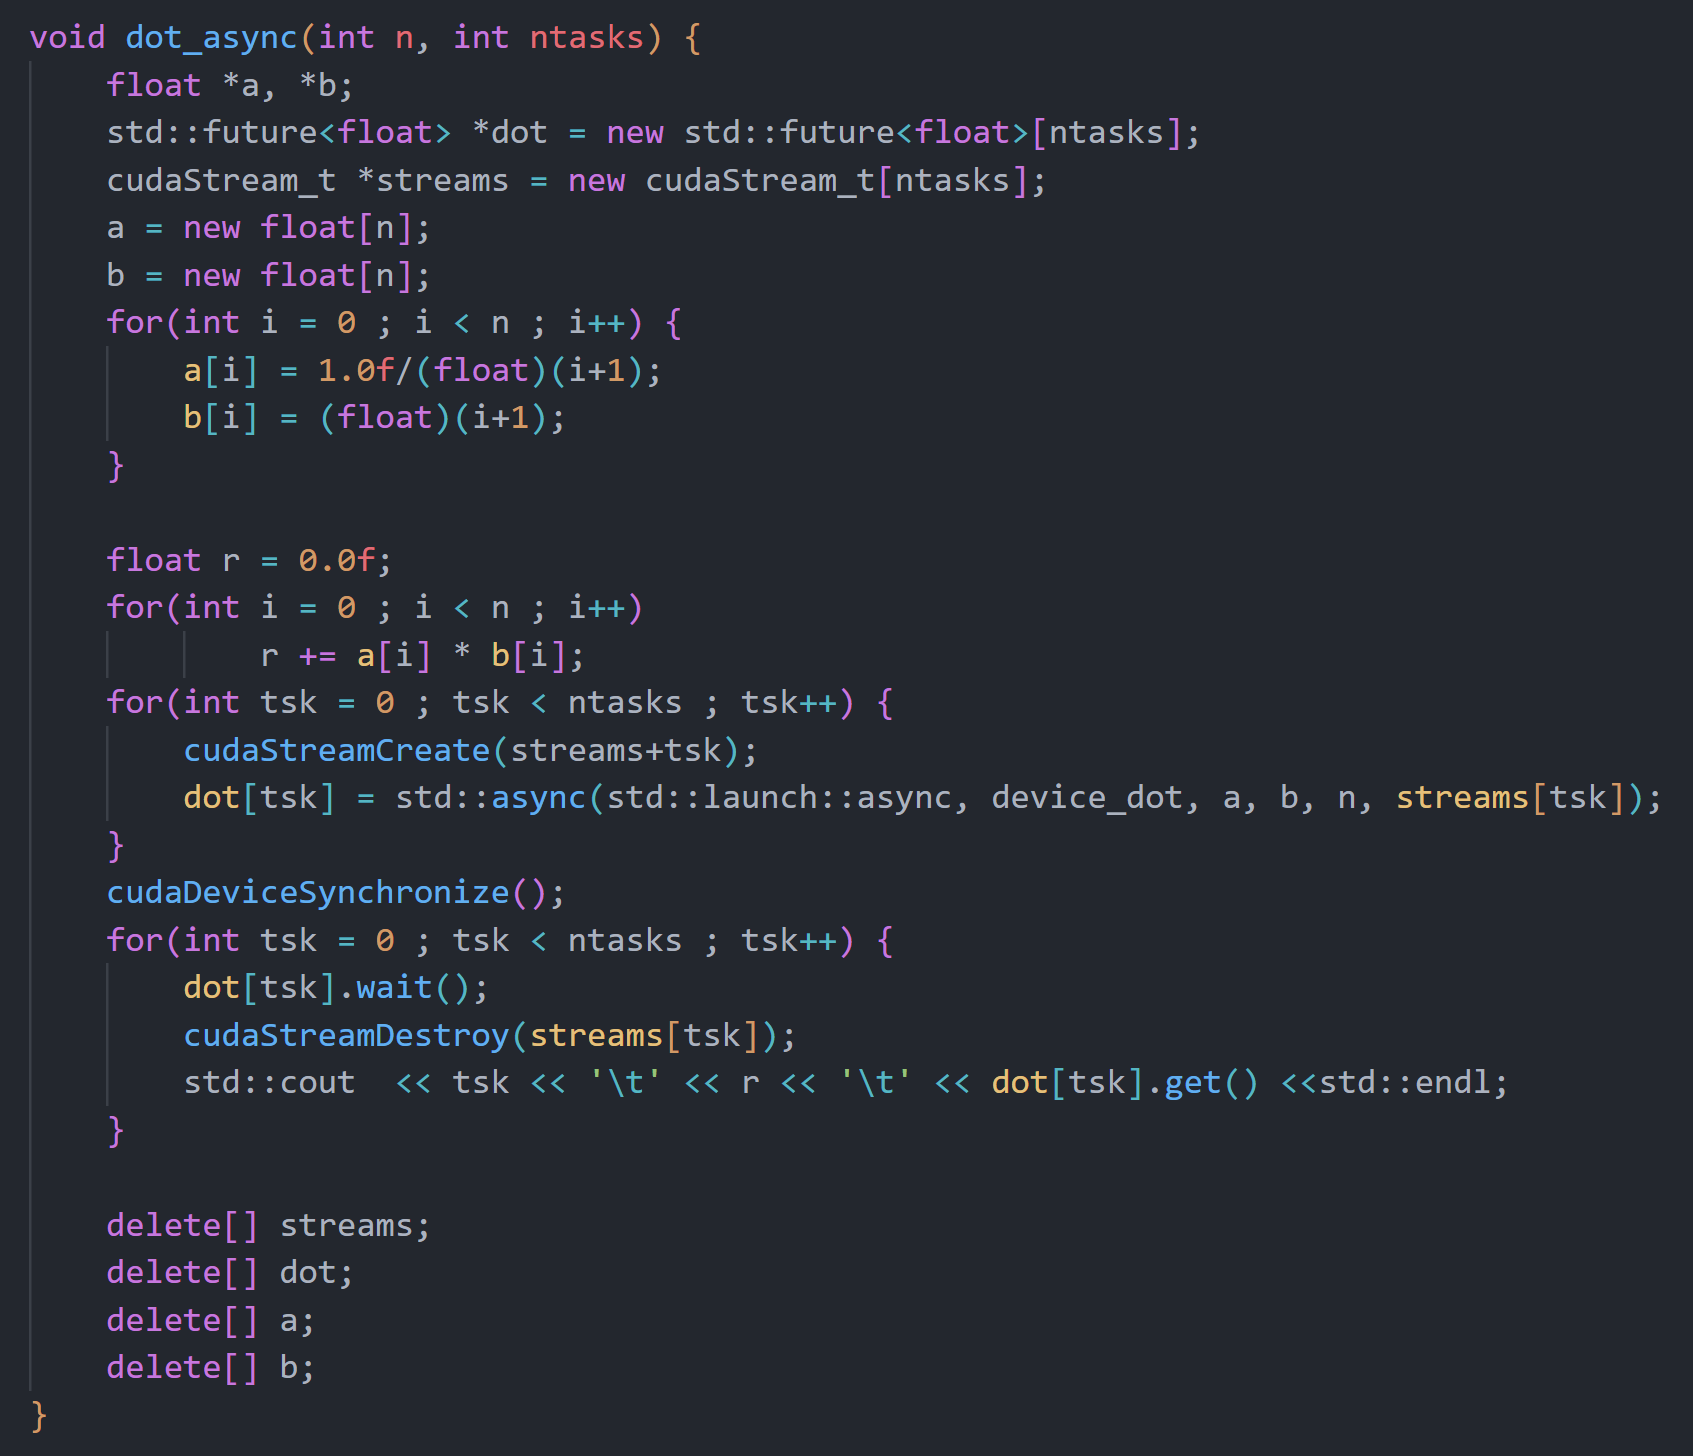
\includegraphics[width=\textwidth]{launch_dot.png}
    \caption{Exécution asynchrone sur le CPU.}
    \label{fig:launch_dot}
\end{figure}
        \end{minipage} & 
        \begin{minipage}{0.45\textwidth}
            \begin{itemize}
                \item<+-> Chaque grille de calcul est appelée dans un processus CPU différent.
           \end{itemize}
        \end{minipage}
\end{tabular}
\end{block}
\end{frame}
\begin{frame}
    \frametitle{Parallélisme dynamique}
\begin{block}{Grilles filles}
 \begin{itemize}
    \item<+-> Une grille de calcul peut en exécuter une autre.
    \item<+-> Un seul processus est responsable du lancement de la grille fille.
    \item<+-> Une grille mère ne peut se terminer avant ses enfants.
    \item<+-> En dehors du flux par défaut, on peut utiliser les flux prédéfinis suivants~:
    \begin{itemize}
        \item<+-> \texttt{cudaStreamFireAndForget}. La grille fille n'est pas synchronisée à sa mère (sauf en fin d'exécution), ni à d'autres enfants.
        \item<+-> \texttt{cudaStreamTailLaunch}. La grille fille est lancée à la fin de l'exécution de la mère. Les enfants se synchronisent entre eux dans l'ordre
        d'appel.
    \end{itemize}
 \end{itemize} 
\end{block}
\end{frame}\begin{frame}
    \frametitle{Parallélisme dynamique}
    \begin{block}{Réduction parallèle}
        \begin{tabular}{cc}
             \begin{minipage}{0.45\textwidth}
      \begin{figure}[htbp]
         \centering
        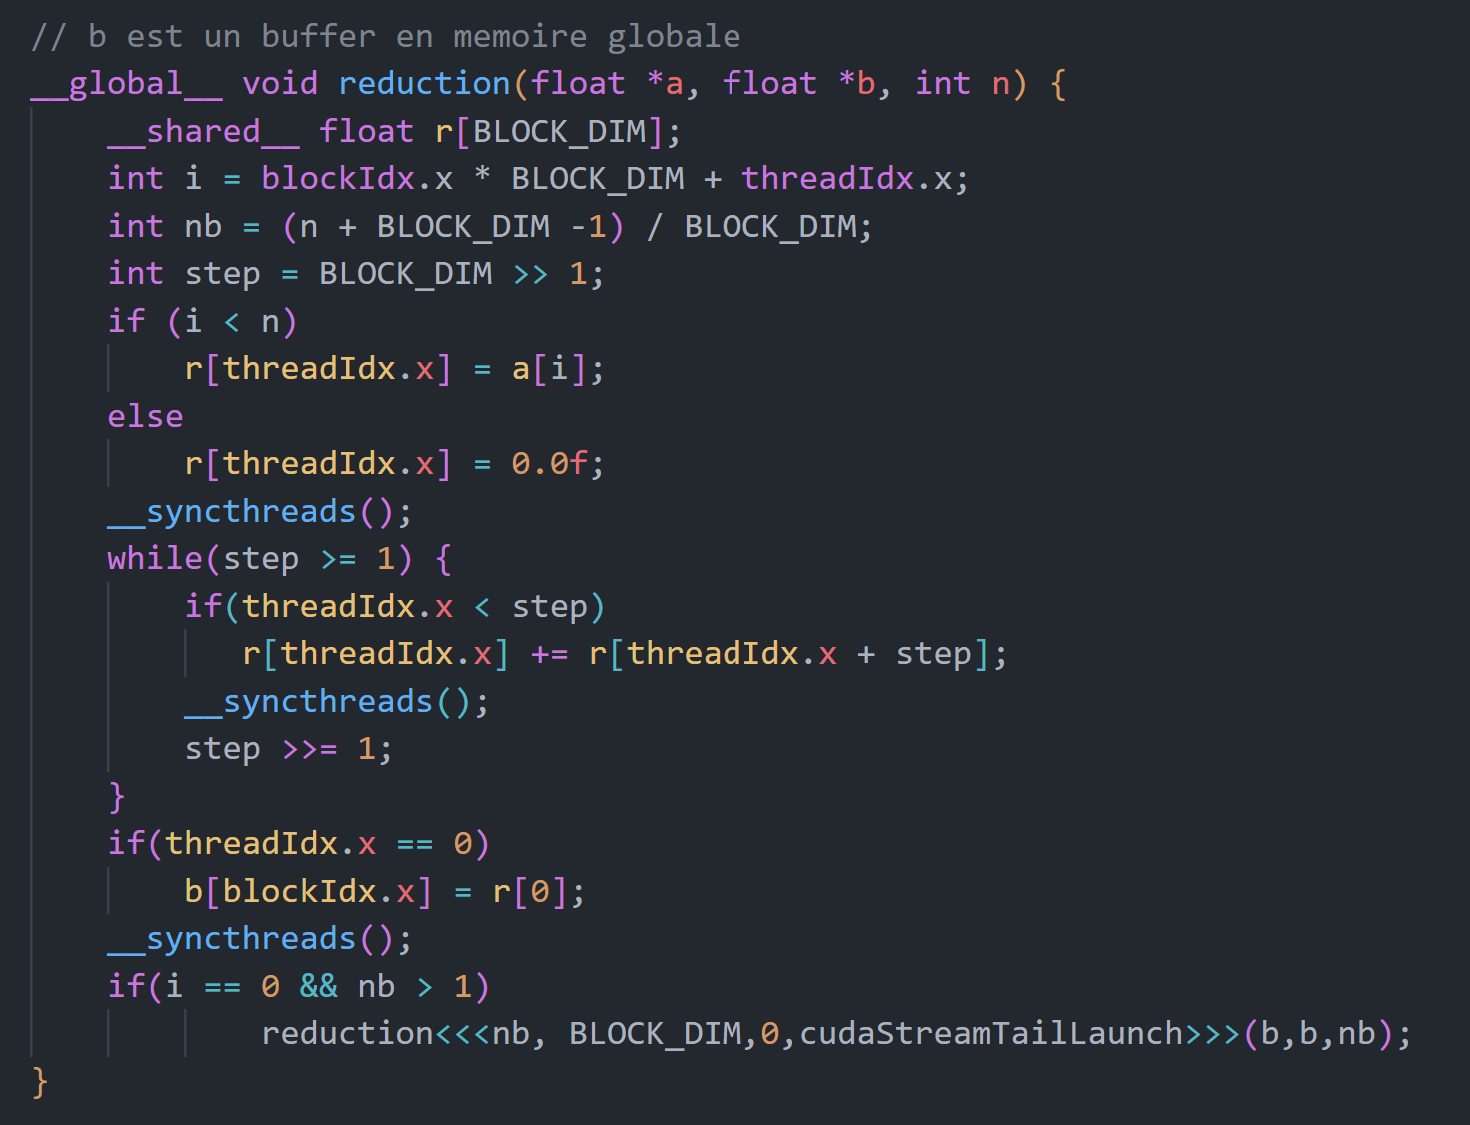
\includegraphics[width=\textwidth]{reduction.png}
         \caption{Création de grilles filles.}
         \label{fig:reduction}
     \end{figure}
             \end{minipage} & 
             \begin{minipage}{0.45\textwidth}
                 \begin{itemize}
                     \item<+-> Le flux \texttt{cudaStreamTailLaunch} garantit l'ordre d'exécution.
                     \item<+-> Il faut des options de compilation spéciales (code relogeable).
                \end{itemize}
             \end{minipage}
     \end{tabular}
     \end{block}
\end{frame}